\documentclass{beamer}
\setbeamertemplate{navigation symbols}{}
\usepackage[catalan]{babel}
\usepackage[utf8]{inputenc}
\usepackage{ragged2e}
\usepackage{tikz}
\usepackage{amsmath}
\usepackage{amssymb}
\usepackage[utf8]{inputenc}
\usetheme{Warsaw}
%\usepackage{lstlisting} %para poner código es este y el de abajo...
%Warsaw
%Antibes
\usepackage{minted}
\usebackgroundtemplate{includegraphics[width=paperwidth,height=paperheight]{}}

\usepackage{pstricks} % modificar tamaño imgane de fondo

\usetikzlibrary{decorations.pathmorphing}
\usetikzlibrary{arrows,positioning,shapes,fit,calc}
\usepackage[most]{tcolorbox}
\usepackage{xcolor}
\usepackage{graphicx}


\title{Criptografía y \TeX}
\subtitle{Trabajo de investigación} 

\title{Criptografía y \TeX}
\subtitle{Trabajo de investigación} 
\author{Marina Fabregat Expósito \\ Tutor: Artur Arroyo}
\institute{Colegio Sant Josep Obrer}
\date{Curso: 2020-2021 \\ 2º Bachillerato A}


\begin{document}

\definecolor{1}{HTML}{FF4B1F}
\definecolor{2}{HTML}{FF9068}
\definecolor{3}{HTML}{EECDA3}
\definecolor{4}{HTML}{EF629F}
\definecolor{5}{HTML}{2980B9}
\definecolor{6}{HTML}{2C3E50}
\definecolor{7}{HTML}{C2E59C}
\definecolor{8}{HTML}{64B3F4}
\definecolor{9}{HTML}{8E9BAE}
\definecolor{gradient1}{HTML}{FEAC5E}
\definecolor{gradient2}{HTML}{C779D0}
\definecolor{gradient3}{HTML}{4BC0C8}
\definecolor{caribbeangreen}{rgb}{0.0, 0.8, 0.6}

\frame{\titlepage}

\begin{frame}
    \frametitle{Índice}
        \tableofcontents
\end{frame}

\section{Introducción}
\subsection{Motivaciones y objetivos}

\begin{frame}
    \frametitle{Introducción}
        \framesubtitle{Motivaciones y objetivos}
        \begin{columns}[t]
        \column[t]{0.45\textwidth}
         \textbf{Motivaciones:}
         
\begin{itemize}
    \item  Personales
    \item 
\includegraphics[scale=0.05]{upf.png}
\end{itemize}
        
        
       
          \column[t]{0.45\textwidth}
          \textbf{Objetivos:}
          \begin{itemize}
              \item Campo profesional 
              \item Profundizar en el campo de la criptografía
              \item Aprender a utilizar \LaTeX
          \end{itemize}
        \end{columns}
 
\end{frame}
\subsection{Hipótesis}
\begin{frame}
\frametitle{Introducción}

    \framesubtitle{Hipótesis}
     \begin{block}{Hipótesis 1} 
        Verificar si soy capaz de comprender los diferentes métodos de criptografía clásica.
    \end{block}
     \begin{block}{Hipótesis 2} 
        Verificar si soy capaz de aprender a utilizar \LaTeX.
 \end{block}
    
\end{frame}
   
       




\section{Desarrollo del trabajo}

\subsection{Metodología y trabajo de campo}


\begin{frame}
\frametitle{Desarrollo del trabajo}
    \framesubtitle{Metodología y trabajo de campo}
    

  
  \begin{block}{Criptografía}
  
  
   \end{block}
   Ejemplo de cifrado de Hill digrámico con clave y mensaje en claro:  

   
   \begin{equation*}
    C= \left(
    \begin{array}{cc}
    7 & 4 \\
    13 & 17
    \end{array}
    \right);\text{ M = UN}
\end{equation*}
   \small
   \begin{equation*}
    \left(
    \begin{array}{cc}
    7 & 4 \\
    13 & 17
    \end{array}
    \right) * \left(\begin{array}{c}
    21 \\
    13
    \end{array}
    \right)=\left(\begin{array}{c}
    199 \\
    494
    \end{array}
    \right) = \left(\begin{array}{c}
    10 \\
    8
    \end{array}
    \right) mod \; (27) \Rightarrow \left(\begin{array}{c}
    K \\
    I
    \end{array}
    \right)
\end{equation*}
\end{frame}



\begin{frame}
      \begin{block}{\LaTeX}
  \begin{itemize}
      \item 
\includegraphics[scale=0.05]{overleaf.png} \begin{itemize}
          \item \LaTeX
          \item Beamer
      \end{itemize}
  \end{itemize}
  \end{block}
  
 %----------------------
 \begin{tikzpicture}
\shade[left color=gradient1, right color=gradient3, middle color = gradient2] (0,0) rectangle (3,2);
\end{tikzpicture}  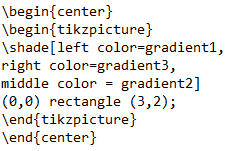
\includegraphics[scale=0.7]{color.png}
 
 %-------------------
\end{frame}

\begin{frame}
\begin{columns}[]
\column[t]{0.45\textwidth}
\begin{equation*}
        \begin{split}
            C^{-1} &= \frac{(Adj(C)^{T})}{\mid C \mid}\\
            C^{-1} &= \frac{1}{39} \left(
        \begin{array}{cc}
            8 & -15 \\
            -7 & 18
        \end{array}\right)\\
            C^{-1} &=  \left(
        \begin{array}{cc}
            8/39 & -5/13 \\
            -7/39 & 6/13
        \end{array}\right)
        \end{split}
    \end{equation*}
\column[t]{0.45\textwidth}

      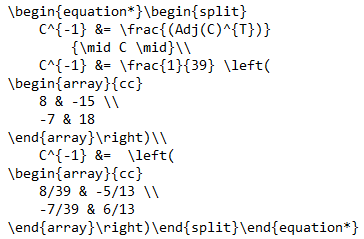
\includegraphics[scale=0.6]{matrizz.png}
  
\end{columns}
      
\end{frame}






\subsection{Problemas y soluciones}


\begin{frame}
\frametitle{Desarrollo del trabajo}
   \framesubtitle{Problemas y soluciones}
 \begin{center}
         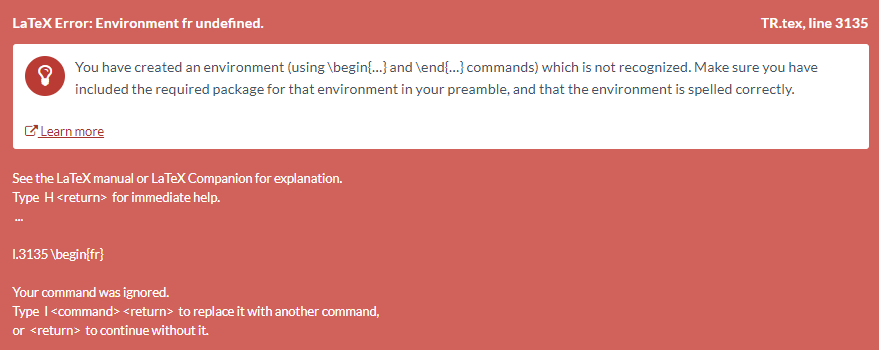
\includegraphics[scale=0.45]{error.png}
   \end{center}
   
   
\end{frame}

\section{Conclusiones}

\begin{frame}
\frametitle{Desarrollo del trabajo}
    \framesubtitle{Conclusiones}
    
    \begin{center} 
    
   \textbf{ Criptografía clásica} 
\includegraphics[scale=0.05]{tick.png}
    \vfill
    
    
         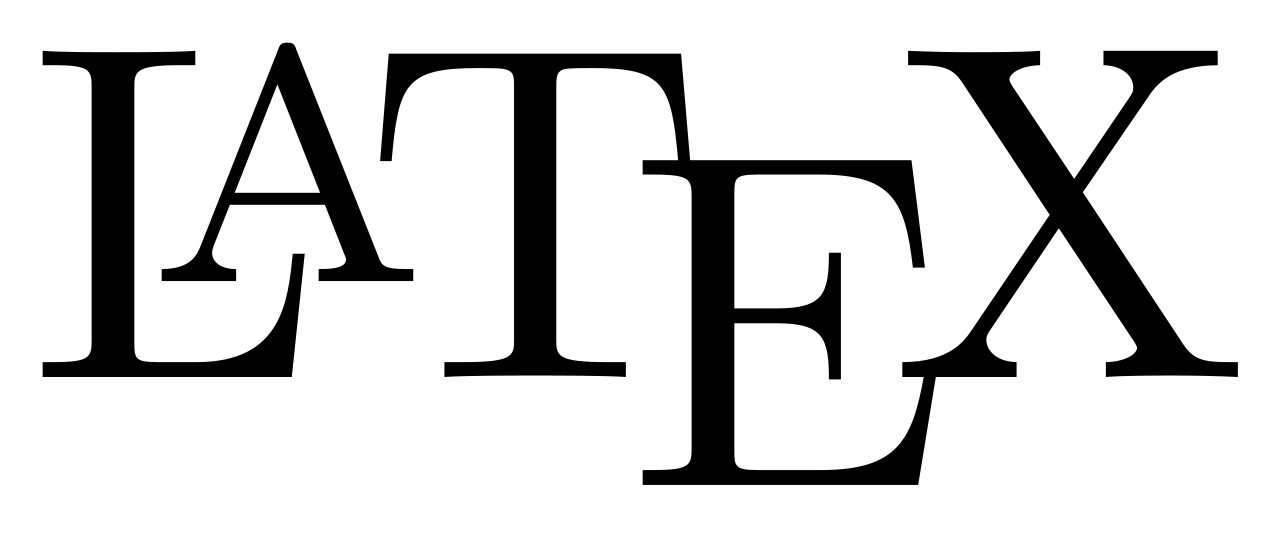
\includegraphics[scale=0.05]{latex.png} 
\includegraphics[scale=0.05]{tick.png} 
    \end{center}
\end{frame}


\end{document}